\section{Motivation}

The field of 3D computer graphics has always been a fascinating subject to me....
...image processing in computer vision...
...high interest in historical topics, because member of citizens association and representative of settlement, thus learning a lot about interesting historical facts and development of culture. For example old railway station in district Langwasser has formerly been used for deportation of people after start of the second world war.
...

\section{Initial project specification}

The idea for this research started with the personal concern of reconstructing a historical site like the old railway station in Langwasser in its historic state. Due to the fact that this railway station has never been fully finished and therefore poor historical documentation, a 3D reconstruction wouldn't be complete. Luckily the famous Pellerhaus was the perfect candidate for this research. After its destruction during World War II, it was rebuilt quite differently to the original state. While the inner courtyard is almost finished with reconstruction at the time of this writing, the facade is still looking modern. At that point, it was clear that the main research topic is going to examine ways to reconstruct the Pellerhaus in its historic state.
A more concrete specification was defined by considering how this is going to be done. The current state of the building has to be captured with laser scanning technology to get the correct measurements from the real world reference. This point cloud data needs to be processed then. To do so, a custom software is required to be written, which can read a file format exported from the proprietary Faro SCENE application, create a panoramic image representation of the data, use it to generate a 3D mesh and export this mesh to a widely supported file format. This research will mostly rely on the open source software Blender to model and animate the historic state of the Pellerhaus, thus it is crucial to provide a compatible output to be used as a basis for the design process. By creating a surface from the point samples, a bug in Blender, which is making it not capable of displaying or rendering colored point clouds\parencite[see][p10]{webBlenderArtistsPointCloudSupport}, this research will overcome this problem. The goal of this research is to get a 3D model of the Pellerhaus in its historic state from 1605 by utilizing panoramic projections as described before.


\section{Project schedule}

This project is divided into two phases. The first phase is developing the software for converting laser scanner point clouds as 3D panorama meshes. The second one is designing the historic 3D model from this initial mesh.

This is visualized in the following GANTT chart:

\definecolor{RoyalBlue}{RGB}{92,102,149}
\definecolor{OliveGreen}{RGB}{51,151,102}
\definecolor{Maroon}{RGB}{180,20,53}
\begin{ganttchart}[
x unit=1.3cm,
y unit title=0.7cm,
y unit chart=0.8cm,
vgrid,
time slot format=isodate-yearmonth,
compress calendar,
title/.append style={draw=none, fill=RoyalBlue!50!black},
title label font=\sffamily\bfseries\color{white},
title label node/.append style={below=-1.6ex},
title left shift=.05,
title right shift=-.05,
title height=1,
bar/.append style={draw=none, fill=OliveGreen!75},
bar height=.6,
bar label font=\normalsize\color{black!50},
group right shift=0,
group top shift=.6,
group height=.3,
group peaks height=.2,
bar incomplete/.append style={fill=Maroon}
]{2015-01-15}{2015-07-15}
\gantttitlecalendar{year, month=shortname} \\
\ganttbar[
progress=100,
bar progress label font=\small\color{OliveGreen!75},
bar progress label node/.append style={right=4pt},
bar label font=\normalsize\color{OliveGreen},
name=pp
]{Laser Scanning}{2015-01-15}{2015-01-25} \\
\ganttset{progress label text={}, link/.style={black, -to}}

\ganttgroup{Software development}{2015-02-15}{2015-03-01} \\
\ganttbar[progress=100, name=T1A]{Import}{2015-02-15}{2015-02-18} \\
\ganttbar[progress=15]{Processing}{2015-02-19}{2015-02-25} \\
\ganttbar[progress=10]{Export}{2015-02-26}{2015-03-01} \\

\ganttgroup{Video production}{2015-04-01}{2015-06-01} \\
\ganttbar[progress=0, name=T2A]{Modeling}{2015-04-01}{2015-05-01} \\
\ganttbar[progress=0]{Animation}{2015-05-01}{2015-06-01} \\

\ganttset{link/.style={OliveGreen}}
\ganttlink[link mid=.4]{pp}{T1A}
\ganttlink[link mid=.159]{pp}{T2A}
\label{tab:project_schedule}
\end{ganttchart}


\section{State-of-the-art methods for 3D reconstruction}

There are several methods that allow for the generation of 3D meshes from various data. One can either use several still images or videos, sample the real world with modern sensor technology. This is described as follows:

\subsection{Light Detection And Ranging (LiDAR)}

The term Light Detection And Ranging (in short LiDAR) is commonly used with high precision applications, such as scanning and mapping. It uses a laser beam emitter and receiver. The time between sending a signal and receiving it is measured and multiplied by the speed of light. This returns the meters the light traveled from the emitter to the obstacle and back. Dividing this distance by two yields the range to the obstacle in meters.\parencite[see][p8-9]{dp_lidar}

As this only gives the meter to one specific point, it is necessary to keep measuring from different viewpoints. This can be done by rotating the scanning device horizontally and vertically simultaneously. To keep cables from winding up by using two motors, devices usually use only one motor for the horizontal and a flat mirror on an elliptical mount for the vertical rotation. That way it is possible to sample a lot of points around the device position quickly and effectively.

In this work the LiDAR scanner Faro Focus 3D is being used. It is capable of capturing 976,000 points per second with a vertical and horizontal field of view of 305 and 360 degrees, respectively\footnote{Techsheet Faro Focus 3D: http://www2.faro.com/site/resources/share/944}. For allowing a better registration it can also use GPS for localization and a barometer for height measurement. The measured points can be colored with a built-in camera of around 70 Megapixels. The price for the Focus 3D totals at 61,404.37 Euro\footnote{http://surveyequipment.com/faro-focus-3d-x-330-laser-scanner/}.

\begin{figure}[h]
	\centering
	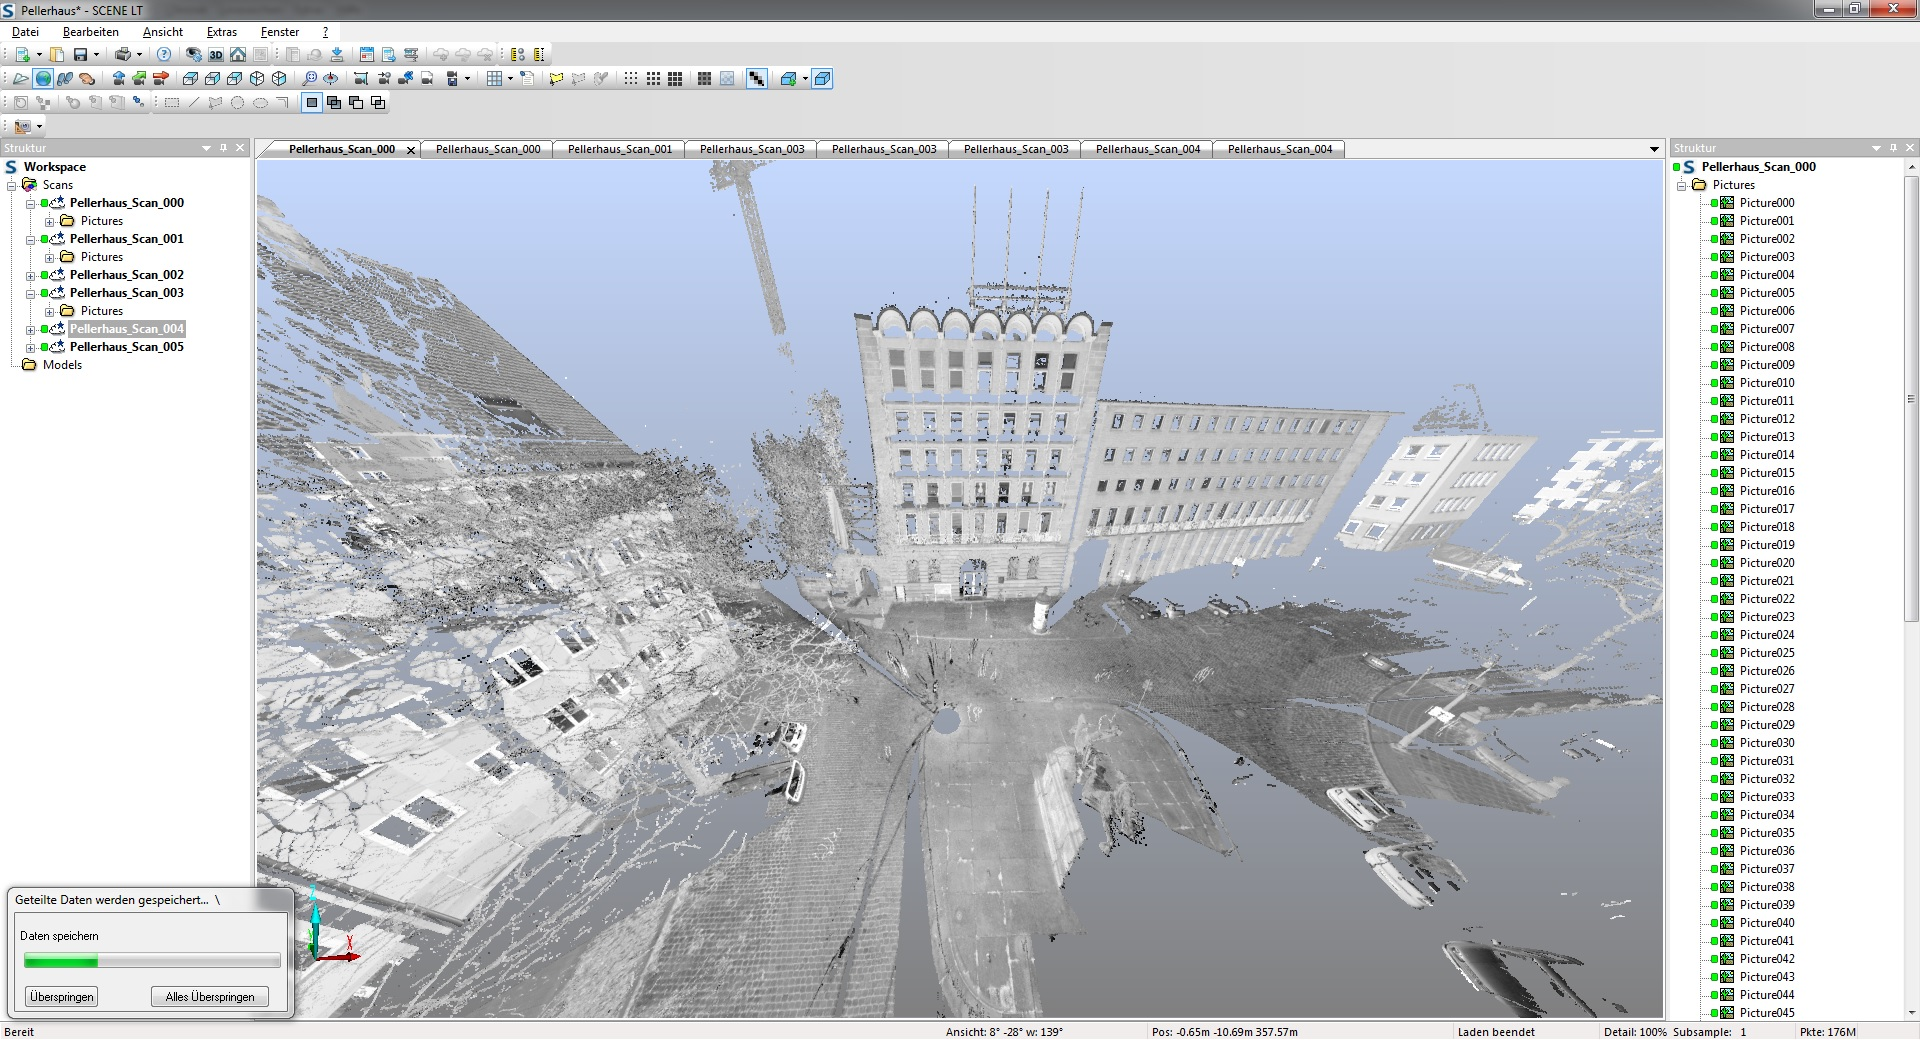
\includegraphics[scale=0.25]{Pellerhaus_FirstGlance.jpg}
	\caption{LiDAR Scanner Point Cloud of the Pellerhaus}
	\label{fig:LiDAR_PointCloud}
\end{figure}

Besides using a stationary device, portable devices are also available. Recently a new technology has been revealed by Csiro and is called \textit{Zebedee}. This handheld laser scanner can be used in challenging environments where a stationary device would require several scans to cover the whole area (e.g. caves, staircases) while the operator is walking. It samples over 40,000 range measurements every second and consists of a 2D laser scanner mounted on a spring system\footnote{http://www.csiro.au/Organisation-Structure/Divisions/Computational-Informatics/Zebedee-3D-mapping.aspx}. Especially the visual effects field has a great use for this device, since the environments can vary a lot during video shootings and a 3D mesh representation is ubiquitous today. The price for the ZEB1 handheld laser scanner is 17,000 Euro\footnote{Source: Personal contact to sales team}.

Although measuring with laser technology can be found in household devices as an alternative for tape measuring, it is still quite complicated to reverse engineer such devices to get the raw distance reading. Fortunately a group of engineers tried to bridge the gap by starting a crowd funding campaign for a low-cost laser range finder, called the LiDAR-Lite\footnote{http://pulsedlight3d.com/}. It has a total range of 40 meters with a resolution of 1 cm. During this research this sensor is being used with a custom arduino build to examine how it can be used as a cheap alternative to the examples mentioned in the beginning. The price for one module is at 82 Euro.

\subsection{Ultrasonic}

In contrast to LiDAR, most ultrasonic sensors are cheap, but generally are not used for higher distances at several tens of meters (though, there are products for a range higher than 100 meter\footnote{VEGAPULS 69: http://www.vega.com/downloads/AL/DE/34137-DE.pdf}). The reason for this is that sound is usually affected stronger by environmental properties than light\footnote{http://www.sensorsmag.com/sensors/acoustic-ultrasound/choosing-ultrasonic-sensor-proximity-or-distance-measurement-825}. Due to this they are often used for shorter distances e.g. for near field obstacle recognition in robotics or in small desktop laser scanners\footnote{https://www.youtube.com/watch?v=saWWhEYQxTg}. Typical ultrasonic sensor modules with a maximum range of around 5 m can be purchased for 5 Euro already.



\subsection{Photogrammetry}

Photogrammetry (also referred to as multi-view reconstruction) is a technique from the Computer Vision field and presents a cost-effective alternative to laser scanning. A real 3D object can be reconstructed as a virtual 3D model by using photographs of the scene and feeding them into such software. This works by detecting image features (for example by using Harris Corner Detector or SIFT algorithms), matching those between image pairs, computing the respective camera positions and re-projecting the reconstructed 3D points to get a point cloud representation of the real photograph\parencite[compare][p29]{bookProgrammingComputerVisionwithPython}.
The computer vision algorithms get better each day and there is plenty of software using them.

\begin{figure}[h]
	\centering
	\begin{subfigure}[b]{0.3\textwidth}
		\centering
		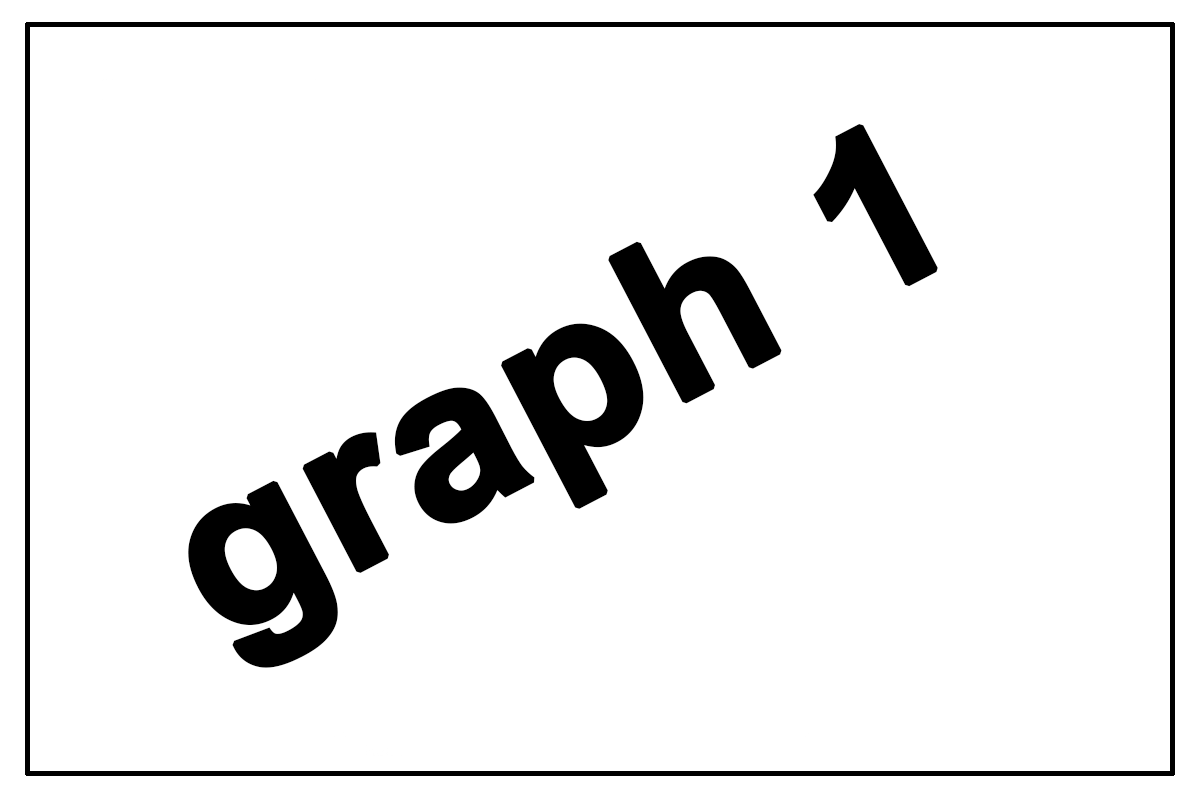
\includegraphics[width=\textwidth]{graph1.png}
		\caption{$OpenSource: Visual SFM + Meshlab$}
		\label{fig:visualsfm meshlab}
	\end{subfigure}
	\hfill
	\begin{subfigure}[b]{0.3\textwidth}
		\centering
		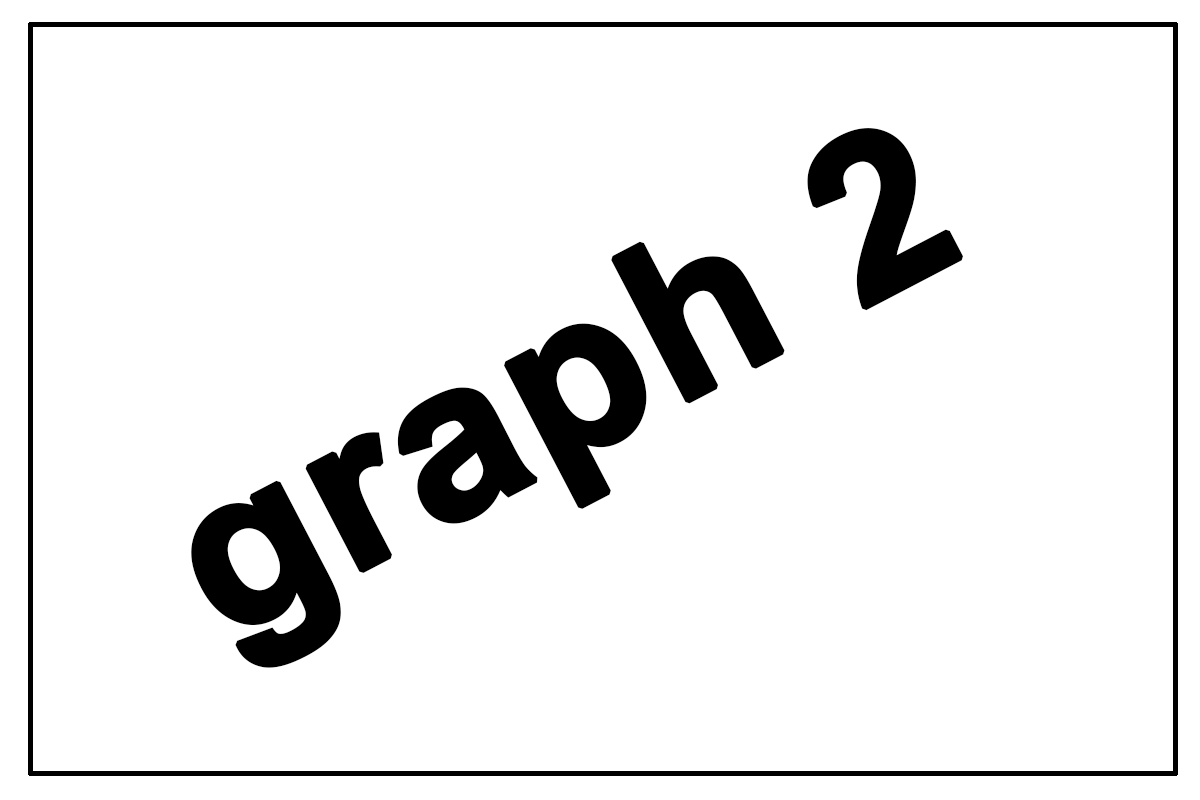
\includegraphics[width=\textwidth]{graph2.png}
		\caption{$Free: Autodesk 123D Catch$}
		\label{fig:123dcatch}
	\end{subfigure}
	\hfill
	\begin{subfigure}[b]{0.3\textwidth}
		\centering
		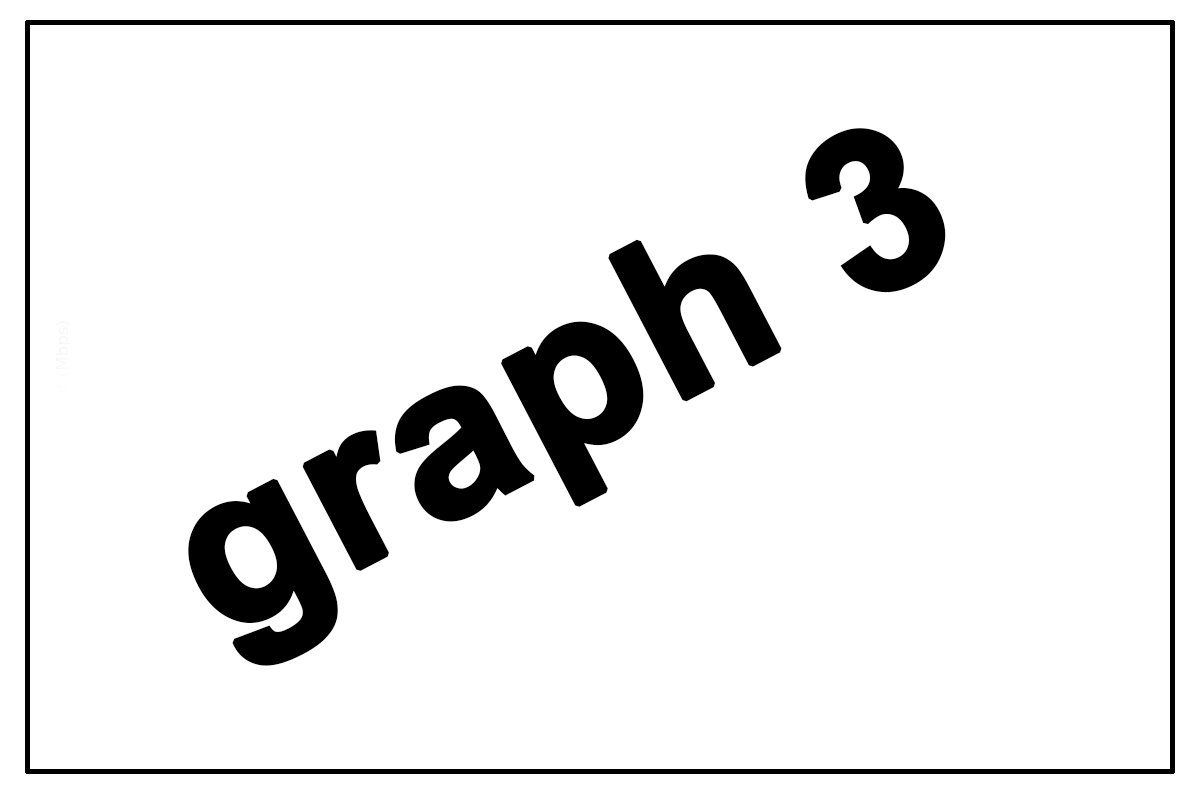
\includegraphics[width=\textwidth]{graph3.png}
		\caption{$Commercial: Agisoft Photoscan Pro (Demo)$}
		\label{fig:photoscan pro}
	\end{subfigure}
	\caption{Multiview Reconstruction from historic stereo pairs}
	\label{fig:multiview reconstruction historic stereo}
\end{figure}

Photogrammetry will be used in this project to try reconstructing surfaces from historical images. Fortunately stereographic image pairs are provided through the Altstadtfreunde Nürnberg e.V. By matching the laser scanner data with the Photogrammetry output a good groundwork is expected to be done for the final surface reconstruction.

\subsection{Google Maps (R) }

The commercial application allows viewing cities from the sky with a rough representation of 3D building shapes\footnote{https://www.youtube.com/watch?v=5iolZU8LwPU}. While this service had gray boxes some years ago, today the visualization is getting more accurate. It is possible to see small details with better modeled and textured buildings.

\subsection{Open Street Map (R) }

The open source alternative to the commercial service above offers the basic functions for map viewing and navigation. OpenStreetMap (OSM) offers very detailed access to its data, like boundaries, streets and building footprints. That way it is possible to extract simple building shapes\footnote{http://demo.f4map.com/\#lat=49.4559869\&lon=11.0762814\&zoom=18} that can be used in custom software free of charge.

To allow for a better mapping of buildings there are also proposals on an indoor version of OSM\footnote{http://wiki.openstreetmap.org/wiki/Indoor\_Mapping}. Having this data available is a helpful thing for applications such as indoor navigation at railway and subway stations, mobile emergency exit information and robotics.

\subsection{Bavarian State Office for Survey and Geoinformation}

Geodata and city plans are also provided officially through governmental institutions. They provide various types of data, among others historical aerial photographs, digital elevation models (DEM) and also 3D building shapes. For educational purposes (like i.e. this research) they offer a university discount for the data of 25 percent. A usual dataset without any discounts containing 7580 buildings of Langwasser, district of Nuremberg in Germany, costs 1158 Euro\footnote{Personal research}.

\subsection{Autonomous mapping with UAV's and SLAM}

Drones, or unmanned aerial vehicles (UAV's), are getting more popular each day. Most of them are also equipped with a camera which allows for taking pictures or videos from viewpoints a human cannot reach easily. More expensive drones have LiDAR systems attached \footnote{https://www.youtube.com/watch?v=IMSozUpFFkU} which allow - together with the IMU (Inertial Measuring Unit) and GPS (Global Positioning System) to localize it and map its environment. A popular term for this is Simultaneous Localization And Mapping (SLAM).

\subsection{Manual methods}

If all other methods fail, there is still the chance to get a reconstruction done roughly by taking measurements of real objects with measuring tapes or eyeballing. Loading pictures from the front, side and top view into a 3D software can already yield decent results.

\section{Defining the scope of this research}

Although this work uses a combination of several techniques (briefly presented above), the main focus is put on examination if panoramic projection of laser scanner point clouds will be an aid for 3D reconstruction or not. This will be evaluated by using the result from the converter in a real world use case of using the reconstructed mesh in the design process.